\documentclass[11pt,a4paper]{article}
\usepackage{amsmath,amssymb}
\usepackage{graphicx}
\usepackage{setspace}
\usepackage{tikz}
\usepackage[margin=1in]{geometry}
\usepackage{booktabs}
\usepackage{multirow}
\usepackage[numbers]{natbib}
\usepackage{natbib}
\usepackage{parskip}
\usepackage{tablefootnote}
\usepackage[linesnumbered,ruled,vlined]{algorithm2e}
\providecommand{\keywordname}{\textbf{Keywords:}} % Customize how "Keywords:" appears
\newcommand{\keywords}[1]{%
  \par\addvspace{\baselineskip}% Adds some space above the keywords
  \noindent\keywordname\enspace\ignorespaces#1 % Displays "Keywords:" followed by the actual keywords
}
\newcommand{\citeboth}[1]{\citeauthor{#1} \citep{#1}}


\usepackage[
    colorlinks=true,      
    linkcolor=green,       
    citecolor=blue,       
    urlcolor=blue,        
]{hyperref}


\title{Investigating the Impact of Macroeconomic Indicators 
on the FTSE 250 Index Using Machine Learning Methods}
\author{Mateen Khan}
\date{\today}

\begin{document}

\maketitle

\begin{abstract}
    This study investigates the impact of the Consumer Price Index, Bank of England Base Rate, US Dollar (USD) and British Pound Sterling (GBP) exchange rate and the M3 money supply measure on the FTSE 250 index, and assesses the effectiveness of radial basis function neural networks as a tool to forecast the price of the FTSE 250 index based on the same set of macroeconomic indicators. This study shows quantitative estimates for the long-term and short-term impacts of the aforementioned macroeconomic indicators on the price of the FTSE 250 index, and demonstrates the effectiveness of radial basis function neural networks as a short-term forecasting tool for the price of the FTSE 250 index, thus providing an alternative to econometric forecasting models.

    \keywords{Macroeconomic indicators; Stock market; FTSE 250 Index; Autoregressive Distributed Lag
    (ARDL) model, RBF Neural Network; Time-series forecasting}
\end{abstract}

\section{Introduction}

The stock market has played a central role in the economic and political ascent of many nations ever since its inception [1].  However, whenever stock market instabilities have arisen in history they have had far-reaching destabilising effects. The Mississippi Bubble was an early example of the inherent dangers within stock markets in the form of speculative bubbles [2]. In this particular case, the stock market crashed as result of an unsustainable rise in share prices fueled by speculation, leading to panic selling, a collapse in confidence, and a massive financial meltdown that rippled through the entire French economy.. Another example is the bursting of the dot-com bubble which had a profound impact on the stock market, leading to a significant crash, particularly in technology stocks. It triggered a severe stock market crash by leading to a rapid sell-off of overvalued tech stocks, which then spread to the broader market. The collapse of key companies, along with forced selling due to margin calls, and the widespread loss of investor confidence created a downward spiral that devastated the stock market. 

Nevertheless, stock markets provide essential benefits by allowing companies to raise capital, offering investment opportunities for individuals, and supporting economic growth through efficient capital allocation. They enhance corporate governance through transparency and accountability, facilitate price discovery and market liquidity, and contribute to government financing through taxes.(Shahbaz et al., 2016). 

The stock market is highly sensitive to macroeconomic indicators because these indicators provide insights into the overall health and direction of the economy. Stock markets react to macroeconomic indicators because these signals help investors anticipate future economic conditions, corporate profits, and investment returns. Positive indicators tend to boost stock prices, while negative indicators can lead to declines in stock prices.

The significance of this study is to quantify the effects of macroeconomic indicators on the stock market as well as assessing the use of these indicators to forecast stock prices over the long-term and short-term, both useful to economic policy makers and stock market investors respectively.

A key task which economic policy makers and investors undertake is to understand and predict how economic changes influence stock market behaviour, which is critical for making informed policy and investment decisions. This modelling of the impact of macroeconomic indicators on stock markets is typically achieved by a variety of methods: statistical analysis, econometric modelling, scenario planning, and advanced machine learning techniques. However, it is fraught with challenges that require careful consideration, advanced techniques, and a deep understanding of both economics and financial markets. In particular, there is a challenge to find a subset of macroeconomic indicators which can most accurately capture stock market dynamics. 
In addition, macroeconomic indicator data is of such low-granularity that it precludes the use of certain deep learning neural network methods for prediction purposes.


This study aims to explore the relationship between macroeconomic indicators and stock markets 
through modelling. Its primary objective is to address questions such as how specific 
macroeconomic indicators influence stock market prices in major economies and whether machine 
learning models can substitute traditional econometric models in predicting stock market prices. 
Ultimately, it aims to investigate three aspects of modelling the impact of macroeconomic 
indicators on stock markets: 
\begin{enumerate}
    \item To investigate how macroeconomic indicators influence the FTSE 250 index
    \item To investigate the short-term and long-term effects of macroeconomic variables on the price of the FTSE 250 index
    \item To investigate whether machine learning techniques can provide accurate short-term and long-term forecasts of the price of the FTSE 250 index when using a low-granularity dataset.
   
\end{enumerate}

In order to analyse the dynamic relationship between variables in time series data, this study will employ the Autoregressive Distributed Lag (ARDL) model in conjunction with an Error Correction Model (ECM). By integrating the ARDL model with the ECM, a comprehensive understanding of both the immediate and longer-term relationships between variables is obtained, which is valuable for robust economic analysis and policy-making.
This research also employs radial basis function neural networks to predict the price of the FTSE 250 index. This artificial deep learning network is particularly useful for tasks like function approximation, pattern recognition, and regression when the dataset is of low-granularity.

The remainder of the paper is organised as follows. Section 2 presents a brief review of the literature in this problem space, and explains the rationale behind our selection of macroeconomic variables. Section 3 covers the data utilised in this study. Section 4 outlines the ARDL-ECM model, the methodology, and the results achieved describing the effect of the selected macroeconomic variables on the FTSE 250 index. Section 5 constructs the radial basis function neural network (RBF-NN) model, and presents the results of forecasting the short-term and long-term forecasts for the price of the FTSE 250 Index price movements based on the selected macroeconomic variables. Section 6 concludes the study.

\section{Literature Review}

\subsection{Stock Market-Macroeconomic Relationships}

The findings of \citeboth{ChenRollRoss1986} state that a long-term equilibrium relationship 
exists between stock market prices and relevant macroeconomic indicators. Based on this, 
\citeboth{EngleGranger1987} proposed an econometric approach utilising a causality test and an 
error correction model (ECM) to investigate this relationship. This approach has been used extensively \citep{QuadriMasih, Plíhal2016,olomu2015} to assess the impact of macroeconomic variables on the stock market. 
Other prominent techniques that have been developed include the Johansen cointegration model \citep{YadavKheraMishra2021,Ozcan2012,ChistiShakeelGanai2020} and the Autoregressive Distributed Lag (ARDL) model \citep{khan2018,demir2019,neifar2023}.

The literature investigating the impacts of the selected variables on the stock market is now presented. A discussion on the FTSE250 as the most accurate representation of the UK stock market is also included.

\subsubsection{Inflation}

The Fisher hypothesis states that nominal interest rates adjust to expected 
inflation as firms correctly anticipate inflation 
and adjust prices, implying that markets are efficient and that inflation has no impact on the stock market. This was tested this in the US stock market by \citeboth{jaffe1976}, and
\citeboth{bodie1976} who both found a negative relationship between inflation and stock returns, providing evidence against the Fisher hypothesis.
To account for this,
\citeboth{mogdiliani1979} proposed the Inflation Illusion Hypothesis, 
arguing that investors overestimate the discount rate in valuations, leading to mispricing. 
\citeboth{gultekin1983} and \citeboth{firth1979}, however, found that the relationship between nominal stock returns and inflation in the UK is positive, and that real returns on UK stocks have remained stable even as inflation varied.
Later, \citeboth{hasan2008} provided evidence against this, challenging the Fisher hypothesis and establishing a 
significant causal relationship between the stock market 


\subsubsection{Interest Rate}

Interest rates, being the cost of borrowing, directly impact firms by increasing financing costs, reducing profitability, and lowering growth prospects. For consumers, higher rates raise borrowing costs, leading to reduced spending and demand, which further lowers corporate profitability \citep{boe199section}. 
The empirical research supports this theory. \citeboth{alam2009} found a significant inverse relationship between interest rates and stock prices across multiple countries from 1988 to 2003.
\citeboth{talla2013} observed a negative relationship between interest rates and stock prices on the Stockholm Stock Exchange.
\citeboth{demir2019} reported similar findings for the Turkish Stock Exchange. In the case of the UK, \citeboth{neifar2023} used a Non-Linear ARDL model to find a significantly negative long-run relationship between interest rates and the FTSE100. 
In addition, the flight-to-quality phenomenon that igher interest rates also encourage a shift from stocks to fixed-income 
assets such as bonds. \citeboth{asgharian2016} provided evidence for this in developed stock markets, including the UK. This suggests interest rates 
negative impact the stock market.

\subsubsection{Exchange Rate}

Classical economic theory explains the impact exchange rates have on stock prices through the portfolio balance model. The portfolio balance model indicates that expected currency depreciations lead investors to shift from domestic to foreign assets, decreasing demand for domestic stocks and lowering their prices. 
\citeboth{branson1977} established a bidirectional relation between the exchange rate and stock prices. This was confirmed
in the case of the Turkish Stock Exchange by \citeboth{aydemir2009}. 
Moreover, stock markets often contain multinational firms involved in international transactions. Their profits are strongly influenced by the exchange rate, and consequently so is the stock market price \citep{Wong2018}.
In support of this, \citeboth{khan2018} found that the exchange rate showed a positive relationship with the Karachi Stock Exchange over the long-run, and a negative impact in the short-run. 
In the case of the UK, \citeboth{wong2022} also demonstrated a positive long-run impact by the exchange rate on the stock market.

\subsubsection{Money Supply}

One of the foundational studies on the relationship between the money supply and 
stock market prices was \citeboth{palmer1970}, who analysed the impact of M1 money supply on the S$\&$P 425 Industrial Stock Index. 
He posited that trends in the nation's money stock could lead the 
private sector to adjust wealth portfolios, resulting in 
predictable movements in stock prices. \citeboth{homa1971} further argued that 
stock prices are significantly impacted by the risk-free interest rate, 
which is a function of money supply. This relationship was disputed by \citeboth{pesando1974}, 
who critiqued the theoretical and empirical methodology used in their study. In addition, \citeboth{sorensen1982} and 
\citeboth{bernanke2005} argue that only the unanticipated component of money supply changes 
affects the stock market price. Later research, however, such as \citeboth{bahloul2017}, 
\citeboth{synek2024}, and \citeboth{pícha2017} has found that the price of developed stock markets, such as the US and UK's, is in fact significantly influenced by the money supply. 
The nature of this relationship is disputed and varies across countries. \citeboth{homa1971} established a positive relationship between the 
stock market and the money supply. This was disputed by \citeboth{sellin2001}, who presents a negative theoretical relationship betwen the stock market and money supply. \citeboth{olawale2014} empirically found a significant positive impact by the money supply on stock returns in the US, but a negative one in the case of the UK. 


\subsubsection{FTSE 250 Index}

The FTSE250 has historically been considered a more closer representation of the domestic economy than the FTSE100. Roughly $50\%$ of the earnings of the FTSE250 are from overseas, similar to the S\&P 500. In contrast, nearly $80\%$ of the FTSE$100$'s earnings are from overseas. 
This is reflected in the constitution of the respective indices, with the 
FTSE250 historically resembling the structure of the UK economy more closely than the FTSE100 \citep{ftse250history}.

In spite of this, the FTSE250 has seldom been utilised as the preferred indicator of the UK stock market in the literature,
with the exception of \citeboth{smit2023longrun}, \citeboth{khatri2024impact} and \citeboth{engstrom2006impact} who investigate the effect of variable changes on the FTSE All Share, an index that aggregates the 
FTSE100, FTSE250 and FTSE SmallCap indices. The impact of the four selected variables on the FTSE250 has not yet been empirically studied and 
warrants further investigation.

\subsection{Stock Market Forecasting}

There is a large body of literature regarding stock market price forecasting. First, 
a discussion on the feasibility of such forecasting is presented. Following this, machine learning methods for forecasting are 
discussed.


\subsubsection{Efficient Market Hypothesis}

The Efficient Market Hypothesis proposed in \citeboth{fama1970} argues that stock market prices fully 
reflect all available information. Fama outlined three forms of the EMH:
weak-form, semi-strong form and strong form EMH.
\begin{enumerate}
    \item Weak-form: Future stock prices cannot be predicted based on past prices.
    \item Semi-strong form: Stock prices quickly adjust to reflect all publicly available information including macroeconomic changes.  
    \item Strong-form: Stock markets are perfectly efficient, stock prices reflect all information, both public and private.
\end{enumerate}

The consistent success of various high-profile investors in the decades 
after the development of the EMH has challenged 
its central argument, something acknowledged in the revised formulation of the EMH 
by \citeboth{fama1991}. Furthermore, the empirical research is not in 
agreement on whether the UK stock market is efficient at any of the three levels. 
\citeboth{libberton2010} and \citeboth{rounaghi} give evidence of weak-form efficiency,
however, \citeboth{borges2010}, \citeboth{asghar2023} and \citeboth{bhavsar2015} al provide evidence to reject the EMH. 
Some studies such as \citeboth{rosini2020} even found that the 
efficiency of the FTSE100 and FTSE250 varied over time. Thus, the empirical findings suggest 
that it is not impossible to forecast movements in the 
price of stock indices on the FTSE250 using macroeconomic variables.



\subsubsection{Machine Learning Methods for Forecasting}

In addition to econometric models, machine learning methods, 
particularly gradient boosting machines \citep{gumelar,Liu2024,Chen2023} and artificial and deep neural networks \citep{chen2015lstm,kara2011ann,long2019deep,nelson2017lstm}, have recently emerged as powerful alternatives capable of overcoming the limitations of econometric models. 
They are able to capture complex relationships in financial data \citep{rossi2018ml}, and 
are thereby able to provide more accurate forecasts than ordinary statistical models 
\citep{lapitskaya2021armax}. 


Deep learning methods such as Recurrent Neural Networks (RNNs) and Long Short-Term Memory (LSTM) Neural Networks
have been extensively used for forecasting time series data, 
such as stock market volatility \citep{cho2022forecasting,praveenraj2023} and prices \citep{zhang2022lstm,song2023forecasting,dutta2024hybrid}. The drawback of such 
methods is that they are not suitable for smaller datasets and tend to overfit on the training data
in such datasets \citep{foster1992} or display unstable behaviour during performance \citeboth{lebaron1998}

Radial Basis Function Neural Networks (RBF-NN) are a type of artificial 
neural network that use radial basis functions at each node in the 
activation layer of the network.
The advantage of RBF-NNs lies in their ability to 
operate effectively in extremely volatile financial time-series 
environments \citep{cafferata2019}, their strong ability to 
generalise on such data \citep{sharkawy2020} as well as their efficacy on small datasets \citep{kosarac2022}. 
\citeboth{esfandyari2016}
supports this, using a sample size of 70 and 29 to forecast daily NASDAQ 
index values using an Artificial Neural Network; they achieved a minimum
test $R^2$ of 83$\%$. 

RBF-NNs have been used considerably for stock market forecasting. \citeboth{cao2004} 
used an RBF-NN based on the Optimal Partition Algorithm (OPA) to 
forecast S$\&$P 500 prices. \citeboth{dass2019} use an RBF-NN, with the Back-propagation 
Algorithm (BPA) used instead to tune parameters; their results demonstrate 
that the RBF-NN outperformed a standard feed-forward neural network. 
\citeboth{ji2014} also found that the RBF-NN was able to predict the value 
of the Shanghai Composite Index on a 45 day time-horizon using the closing price, with a mean prediction error of 
1.4387$\%$. Recently, \citeboth{abotaleb2024}
used quarterly data from 2001 to 2023 to model the influence of the economic 
uncertainty index on the quarterly prices of various stock markets including the 
FTSE100 using an RBF-NN. They found that the model 
achieved a relative error of 27.2$\%$ in the case of the FTSE100.

Whilst \citeboth{abotaleb2024}, used quarterly data and a relatively minor economic indicator, the effectiveness of RBF-NNs in stock market forecasting using 
major macroeconomic indicators and coarse-grain time-series has not yet been investigated and presents an area for further 
research. 

\section{Data}

FTSE-250 monthly price data between Oct 1992 to March 2024 has been utilised for this study giving 379 observations.

During the data collection process, it was necessary to deal with an issue raised by the fact that the Bank of England’s Monetary Policy Committee (MPC) 
does not convene on a monthly basis, and are not obligated to 
announce a rate on a regular basis. To address the resulting irregularities the data was adjusted using the following algorithm:

\begin{algorithm}[H]
    \caption{Calculate monthly interest rate}
    \label{alg:interest_rate_adjustment}
    \KwData{Interest rate data adjustments by the Bank of England’s MPC}
    \KwResult{Monthly interest rate data}
    
    \For{each month $m$}{
        \If{$\forall d \in D_m \; \text{(interest rate unchanged)}$}{
            \textbf{Set:} $\text{Rate}_m \leftarrow \text{Rate}_{m-1}$\;
        }
        \Else{
            \For{each day $d_j$ with a rate change}{
                \textbf{Compute:} 
                $W_{int} = \sum_{i_k \in I_m} \frac{i_k  d_{j_k}}{x}$\;
                where $I_m = \{i_1, i_2, \ldots, i_n\}$ is the set of interest rates on days with changes, 
                and $d_{j_k} \leq x$ is the number of days into the month each rate $i_k$ occurs on.
            }
            \textbf{Set:} $\text{Rate}_m \leftarrow W_{int}$\;
        }
    }
\end{algorithm}


\begin{table}[h!]
    \centering
    \caption{Data sources}
    \begin{tabular}{lll}
        \toprule
        \textbf{Variable} & \textbf{Notation} & \textbf{Source} \\
        \midrule
        FTSE 250 Index & FTSE$_{250}$ & Yahoo Finance \\
        Consumer Price Index & CPI & Office for National Statistics (ONS) \\
        USD/GBP Exchange Rate (£) & EXCHG & Federal Reserve of St Louis \\
        Interest Rate ($\%$) & INT & Bank of England \\
        Money Supply (M3) (millions £) & M3 & Bank of England \\
        \bottomrule
    \end{tabular}
\end{table}

Over the period covered by our dataset, the FTSE250 index has 
shown substantial growth, reflecting the structural transition of the UK economy.
It has also experienced significant volatility, highlighting significant market shifts driven by 
various crises such as the Dotcom bubble burst, and geopolitical shocks.

\begin{table}[h!]
    \centering
    \caption{Descriptive statistics}
    \begin{tabular}{lllll}
        \toprule
        \textbf{Variable} & \textbf{Mean} & \textbf{SD} &  \textbf{Min.} & \textbf{Max.}\\
        \midrule
        FTSE 250 Index &  11,013 & 6,162 & 2,520 & 24,102 \\
        CPI Index &  88.4 & 18.0 & 62.8 & 134 \\
        USD/GBP Exchange Rate (£) &  0.659 & 0.085 & 0.483 & 0.883 \\
        Interest rate ($\%$) &  3.21 & 2.52 & 0.1 & 8.4 \\
        Money Supply (M3) (millions £) &  1,861,958 & 971,112 & 494,181 & 3,704,873 \\
        \bottomrule
    \end{tabular}
\end{table}


The USD/GBP exchange rate has exhibited moderate variability, exhibiting the stable relations between 
the two countries. Nonetheless, geopolitical shocks such as the 2008 financial crisis and Brexit both greatly affected the value of the Pound, 
which accounts for the large range. 

The CPI, with an average of 88.36, has 
experienced significant fluctuations, highlighting periods of high inflationary pressure such as in the late 2000s 
near the global financial crisis, and during the onset of the Russia-Ukraine conflict in 2022, and periods of stable, low
inflation such as the early to late 2010s.

Interest rates, have varied widely from $0.1\%$ to $8.4\%$, with a standard deviation of $2.52\%$, reflecting the 
increasing role played by monetary policy in the UK since May 1997 when the Bank of England was given operational responsibility for setting interest rates \citep{king1997changes}. The Bank of England was forced to adjust interest rates 
several times in response to worsening economic conditions, examples being the steep rate cuts during the 2008 financial crisis to stimulate the economy and the gradual rate hikes in response to 
subsequent post-COVID inflationary pressures. 

The M3 money supply has shown substantial variability, ranging from 494,181 to 3,704,873, 
in large part influenced by the various Quantitative Easing (QE) programs implemented by the Bank of England 
in response to the recessions onset by the 2008 financial crisis and the COVID-19 pandemic. These programs aimed to inject liquidity into the economy to stimulate economic activity, thus inflating the overall money supply.

\section{ARDL Model}

Based on the empirical research and characteristics of the UK economy,
the stock market function is defined as:

\begin{align}
    FTSE_{250} = f\biggl(CPI, EXCHG, INT, M3\biggr) \label{eq:implicit}
\end{align}

The study uses an autoregressive distributed lag (ARDL) model in conjunction with 
an error correction model (ECM) to determine 
whether a long-term dependence exists for the FTSE250 and our macroeconomic 
indicators, and if so to quantify the long-run and short-run relationships
between the former and the latter. 

\subsection{Methodology}

Before constructing the ARDL model a natural logarithmic transform is applied
on the variables, this is done because in a log-transformed model,
the coefficients can be interpreted as elasticities (percentage changes). Having done this,
the level at which the variables are stationary is checked.
Various techniques exist for stationarity testing, however in this study the 
Augmented Dickey-Fuller (ADF) unit root test was used. The optimum lag for the variables in the ARDL model was then found using the Schwarz
Information Criterion.

The implicit form \eqref{eq:implicit} is represented in the ARDL model as:

\begin{align*}
    \Delta \text{FTSE}_{250_t} &= \alpha_0 + \sum_{i=1}^{p} \alpha_i \Delta \text{FTSE}_{250_{t-i}} + \sum_{j_{1}=0}^{q_1} \beta_{1j_{1}} \Delta \text{CPI}_{t-j_{1}} + \sum_{j_{2}=0}^{q_2} \beta_{2j_{2}} \Delta \text{INT}_{t-j_{2}} \\
                               & \sum_{j_{3}=0}^{q_3} \beta_{3j_{3}} \Delta \text{EXCHG}_{t-j_{3}} + \sum_{j_{4}=0}^{q_4} \beta_{4j_{4}} \Delta \text{M3}_{t-j_{4}} + \varepsilon_t + \phi_{1} FTSE_{250_{t-1}} \\
                               & + \phi_{2} CPI_{t-1} + \phi_{3} INT_{t-1} +\phi_4 EXCHG_{t-1} + \phi_5 M3_{t-1}
\end{align*}

Here, the intercept term, represents the baseline level of \(\Delta \text{FTSE}_{250_t}\), is given by $\alpha_0$; the 
remaining $\alpha_i$ terms represent the short-run relationships 
between the variables, and $\phi_j$ represent the long-run relationships. 

In the ARDL bounds test, the null and alternate hypothesis are:
 
\begin{align*}
    H_{0}: \phi_i &= \phi_j\\
    H_{1}: \phi_i &\neq \phi_j
\end{align*}

for, $i,j = 1,2,3,4,5$, with $i\neq j$. The F-statistic is computed for the joint
significance of the lagged variables and compared against the critical values
given by \citeboth{pesaran2001} to determine whether cointegration exists, 
and at what significance level. If cointegration exists, then 
the long-run coefficients $\kappa_i$ are estimated to find the cointegration equation:

\begin{align}
    FTSE_{250} = \kappa_0 + \kappa_1 CPI + \kappa_2 INT + \kappa_3 EXCHG + \kappa_4 M3 + \varepsilon \label{eq:two}
\end{align}

Then, an Error Correction Model (ECM) is constructed:

\begin{align*}
    \Delta \text{FTSE}_{250_t} &= \alpha_0 + \sum_{i=1}^{p} \alpha_i \Delta \text{FTSE}_{250_{t-i}} + \sum_{j_{1}=0}^{q_1} \beta_{1j_{1}} \Delta \text{CPI}_{t-j_{1}} + \sum_{j_{2}=0}^{q_2} \beta_{2j_{2}} \Delta \text{INT}_{t-j_{2}} \\
                               & \sum_{j_{3}=0}^{q_3} \beta_{3j_{3}} \Delta \text{EXCHG}_{t-j_{3}} + \sum_{j_{4}=0}^{q_4} \beta_{4j_{4}} \Delta \text{M3}_{t-j_{4}} + \gamma\text{ECT}_{t-1} + \varepsilon_t
\end{align*}

where the error correction term ECT is found by calculating the residual 
produced by \eqref{eq:two}:

\begin{align*}
    ECT_{t-1} = FTSE_{250_{t-1}} - \biggl(\kappa_0 + \kappa_1 CPI + \kappa_2 INT + \kappa_3 EXCHG + \kappa_4 M3 + \varepsilon \biggr)
\end{align*}

The parameter $\gamma$ describes the speed at which short-run deviations from the long-run equilibrium
are adjusted. A negative $\gamma$ implies that there exists a correction mechanism that converges the deviation 
to the long-run equilibrium. To estimate the short-run coefficients, $\alpha_i$ and $\beta_k$, as 
well as the short-run correction speed $\gamma$ OLS regression is used.

\subsection{Results}

First, a natural logarithmic transform was applied on the variables, and 
then conducting the ADF unit root test on the data. The null hypothesis of the 
ADF Unit Root test is that of non-stationarity, and the alternate hypothesis 
is that the variables are stationary.


\begin{table}[h!]
    \centering
    \caption{Augmented Dickey-Fuller (ADF) Unit Root Test\tablefootnote{All of the variables are tested in logarithmic form. The asterisks *, **, ***, and **** denote statistical significance
    at the 1$\%$, 2.5$\%$, 5$\%$ and 10$\%$ significance levels.}}
    \begin{tabular}{lccc}
        \toprule
        \textbf{Variable} & \textbf{Level ADF} & \textbf{First Difference ADF} & \textbf{Stationarity} \\
        \midrule
        FTSE$_{250}$ & $-3.2646^{****}$ & $-6.6892^{*}$ & At first difference \\
        CPI          & $-1.4594$ & $-4.705^{*}$ & At first difference \\
        EXCHG        & $-2.2467$ & $-7.3855^{*}$ & At first difference \\
        INT          & $-2.0946$ & $-4.1156^{*}$ & At first difference \\
        M3           & $-0.70827$ & $-6.3806^{*}$ & At first difference \\
        \bottomrule
    \end{tabular}
\end{table}


Subsequently, the optimum lag of the variables was calculated using the 
Schwarz Information Criterion, to obtain the optimum model 
of ARDL(5, 4, 7, 7, 4). The resulting F-statistic of $4.0798$ was compared against the critical values
given by \citeboth{pesaran2001}, providing evidence of cointegration 
at the $10\%$, $5\%$ and $2.5\%$ significance levels, but not at the $1\%$ 
level.

\begin{table}[h!]
    \centering
    \caption{ARDL Bounds Test Critical Values}
    \begin{tabular}{lcccc}
        \toprule
        \textbf{Order} & \textbf{10$\%$} & \textbf{5$\%$} & \textbf{2.5$\%$} & \textbf{1$\%$} \\
        \midrule
        I(0) & $2.20$ & $2.56$ & $2.88$ & $3.29$ \\
        I(1) & $3.09$ & $3.49$ & $3.87$  & $4.37$ \\
        \bottomrule
    \end{tabular}
\end{table}

The long-run and short-run coefficients were then estimated, and presented 
alonsgide the diagnostic test results which confirm that the model does not
display autocorrelation, heteroskedascity, non-normality and the cumulative 
sum of residuals and squared residuals are both stable, indicating that the 
relationship between the variables has not changed over time. The error
correction term is also given, and it is negative, as expected.

\begin{table}[h!]
    \centering
    \caption{Coefficients Estimates}
    \begin{tabular}{llll}
        \toprule
        \textbf{Variable} & \textbf{Long-Run Coefficient} & \textbf{Variable} & \textbf{Short-Run Coefficient} \\
        \midrule
        FTSE$_{250}$ & $-$ & FTSE$_{250}$ $(-5)$  & $-0.033089$ \\
        CPI & $3.157179$ & CPI $(-4)$ & $-0.921235$ \\
        INT & $-0.1341097^{***}$ & INT $(-7)$ & $-0.034572^{****}$\\
        EXCHG &  $-0.890146^{****}$ & EXCHG $(-7)$ & $0.122318$ \\
        M3 & $-0.1141114$ & M3 $(-4)$ & $-0.527798^{***}$ \\
        Intercept & $-3.447767$ & ECT $(-1)$ & $-0.1001^{**}$ \\
        \bottomrule
    \end{tabular}
\end{table}

\begin{table}[h!]
    \centering
    \caption{Diagnostic Tests}
    \begin{tabular}{llll}
        \toprule
        \textbf{Condition} & \textbf{Test} & \textbf{p-value} & \textbf{Result} \\
        \midrule
        Autocorrelation & Box-Ljung Test & $0.9926$ & No autocorrelation \\
        Heteroskedascity & Breusch-Pagan Test & $0.3635$ & Homoskedascity \\
        Normality & Shapiro-Wilk Test & $3.889$e-$08$ & Normality \\
        CUSUM & CUSUM Test & $-$ & Stable \\
        CUSUM$^2$ & CUSUM$^2$ Test & $-$ & Stable \\
        \bottomrule
    \end{tabular}
\end{table}

The long-term coefficients show that the interest rate and exchange rate
interest rate have significant long-term effects on the stock market price
while money supply and inflation are statistically insignificant. \citeboth{neifar2023}
proposes that this is because deflation, that is the negative movements in the 
CPI, is a statistically significant factor in the movement of the UK stock 
market, but positive movements (inflation) are not. Nevertheless, the positive
coefficient of 3.16, and the negative short-term adjustment, is in line with the expectation from the literature that 
inflation exerts a positive effect on the stock market in the long-term, but a negative 
one in the short-run. 

The insignificant long-term effect of the money supply can be explained by several reasons.
Firstly, as discussed in \citeboth{sellin2001}, it is possible that the FTSE250 is efficient in processing changes in the 
money supply, at least over certain intervals if not always. This would mean anticipated changes in the money supply would not affect the stock market price, only the
unanticipated component of a change in money supply would, as established by \citeboth{sorensen1982} and \citeboth{bernanke2005}. 
It is also possible that the M3 measure is too broad of a measure and includes overly illiquid components that are not as impactful 
on the stock market dynamics. In the short-run we see that the money supply does have a 
significantly negative effect on the stock market, as outlined by \citeboth{olawale2014}. According to \citeboth{sellin2001}, 
this supports the Keynesian argument that a positive money supply shock will lead people to
expect a contraction in future monetary policy. 
This leads to an increase in the demand for funds, which drives up the current rate of interest, in turn
reducing the present value of earnings in the Discounted Cash Flow (DCF) stock valuation model. The effect is a decline in the stock market prices.

Unsurprisingly, the USD/GBP exchange rate is significantly related to the FTSE250's movements. It 
should not be forgotten that, although it is considered to be a more domestic indicator of the LSE, 
at times $50\%$ of the FTSE250's earnings have come from abroad, indicating that 
the value of the Pound has a significant impact on this stock market. 
In the long run, the appreciation of the Pound would increase the relative 
cost of UK exports increases, thereby reducing the 
competitiveness of FTSE250 companies in international markets. This in turn would lower their earnings
and depress the FTSE250. Moreover, foreign investors may view the stronger Pound as a signal of reduced returns on their investments in the UK, which can lead to decreased investment in the FTSE250. 
In the short-term, however, before structural shifts can materialise we see that the
weakening of the Pound has a positive effect. As the USD has been 
the global reserve currency for many decades, the depreciation of the Pound 
against it will lead to increased revenue in Pound terms for FTSE250 companies with substantial overseas operations. This is because their foreign earnings, when converted back into Pounds, will be worth more, potentially increasing profits. The findings 
are in line with \citeboth{neifar2023} and \citeboth{khan2018}.

The interest rate was also found to have significant negative long-term and short-term effects on the stock market, confirming the findings of the extant literature \citep{alam2009,demir2019,neifar2023, talla2013}. 
This can be explained by the fact that higher interest 
rates increase the cost of borrowing for companies, leading to reduced investment 
and lower future earnings potential, in turn depressing stock prices. 
Furthermore, as per the flight-to-quality phenomenon, persistently higher interest rates make bonds and other fixed-income 
investments more attractive relative to stocks, leading investors to shift 
their portfolios away from equities and toward safer assets over time \citep{asgharian2016}. 
In the short term, interest rate hikes immediately decrease the present value of earnings, as per the 
DCF valuation model, and depress prices.

The error correction term 
is negative and statistically significant ensuring that long-run equilibrium 
can be achieved. The adjustment speed of $0.1001$ indicates that 
roughly $10\%$ of the fluctuation in the previous month's price caused by the 
macroeconomic variable movements is adjusted back to the long-run equilibrium in the current month.
However, only increases in the interest rate and money supply are able to 
significantly contribute towards this correction, with $1\%$ increases in the former 
leading to a $-0.03\%$ change in the FTSE250 price 7 months later, and in the case of the latter
a $-0.53\%$ change after a 4-month lag. 

\section{RBF Neural Network}

\subsection{Model Architecture}

\begin{figure}[h]
    \centering
    \hspace{-2.6cm} 
    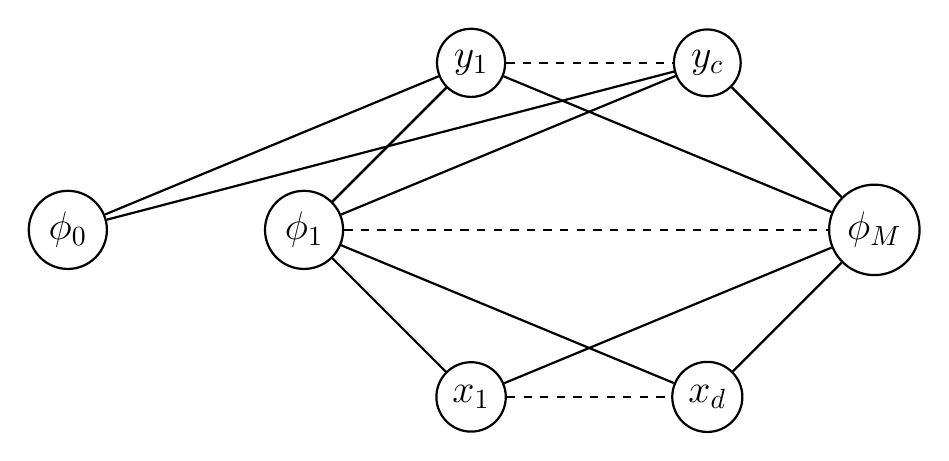
\begin{tikzpicture}[node distance=3cm,
                        thick, 
                        main node/.style={circle, draw, font=\sffamily\Large\bfseries}]
                        
      
      \node[main node] (1) {$y_{1}$};
      \node[main node] (2) [right of=1] {$y_{c}$};
      \node[main node] (3) [below left of=1] {$\phi_{1}$};
      \node[main node] (4) [below right of=2] {$\phi_{M}$};
      \node[main node] (5) [below right of=3] {$x_{1}$};
      \node[main node] (6) [below left of=4] {$x_{d}$};
      \node[main node] (7) [left of=3] {$\phi_{0}$};
      
      
      \draw[thick, dashed] (1) -- (2);
      \draw[thick, dashed] (3) -- (4);
      \draw[thick, dashed] (5) -- (6);
      \draw[thick] (1) -- (3);
      \draw[thick] (1) -- (4);
      \draw[thick] (2) -- (4);
      \draw[thick] (7) -- (1);
      \draw[thick] (7) -- (2);
      \draw[thick] (3) -- (1);
      \draw[thick] (3) -- (2);
      \draw[thick] (3) -- (6);
      \draw[thick] (3) -- (5);
      \draw[thick] (4) -- (5);
      \draw[thick] (4) -- (6);

    \end{tikzpicture}
    \caption{RBF-NN Architecture}
    \label{fig:your_label}
\end{figure}

The exact interpolation problem, which forms the motivation for RBF-NNs, 
involves mapping a $d$-dimensional input space $\boldsymbol{\mathrm{X}}$ to
a $c$-dimensional target space $\boldsymbol{\mathrm{y}}$. The dataset consists of $N$ input
vectors $\boldsymbol{\mathrm{x_n}}$, along with corresponding target 
values $y_n$. The objective is to find a function
  $h(\boldsymbol{\mathrm{x}})$ such that:


\begin{align}
  h(\boldsymbol{\mathrm{x_n}}) = y_n, \quad \text{for } n = 1, \ldots, N
\end{align}

The radial basis function approach 
introduces a set of $N$ basis functions, one for each 
data point. The radial basis function, $\phi(\cdot)$ is some non-linear function of the Euclidean distance
$||\boldsymbol{\mathrm{x}} - \boldsymbol{\mathrm{x_n}}||$. The output of the mapping is then expressed as a linear combination of these basis functions:

\begin{align}
    h(\boldsymbol{\mathrm{x}}) = \sum_{n=1}^{N} w_n \phi(||\boldsymbol{\mathrm{x}} - \boldsymbol{\mathrm{x_n}}||)
\end{align}

By introducing several modifications to the exact interpolation 
procedure, the RBF-NN
model is obtained, as outlined originally in \citeboth{broomhead1988}. 
The RBF-NN mapping takes the following form:

\begin{align}
    y(\boldsymbol{\mathrm{x}}) =  \sum_{j=1}^{M} w_{j} \phi_j(\boldsymbol{\mathrm{x}}) + w_{0}
\end{align}



\begin{align}
    \phi_j(\boldsymbol{\mathrm{x}})  &= f(||\boldsymbol{\mathrm{x}-c_j}||), \quad{j=1\ldots,M}
\end{align}

where $\boldsymbol{c_j}$ is a RBF centre and $f$ is the radial basis function. 


\subsection{Methodology}

The RBF-NN was utilised for both short-term and long-term 
predictions. For short-term forecasting, 
the model was tested over a 5-month horizon, based on the optimum lag calculated earlier, while the long-term predictions spanned 57 months. 
The data was differenced based on the recommendations of the 
unit root tests conducted earlier to achieve stationarity. 

The data was normalised using a z-score normalisation. This is because
neural networks work best with data
that is between a specified range; it ensures that the data is roughly uniformly
distributed between the network inputs and outputs 
(Mendelsohn, 1993, Preprocessing Data for Neural Networks). Following this 
it was necessary to program the RBF-NN into Python. As no specific RBF package exists
in Python, the kernel regression approach outlined by 
\citeboth{bishop1995}, using the GaussianProcessRegressor package in Python.

\subsubsection{The Gaussian Process Regressor}

The Scikit GaussianProcessRegressor is based on the 
standard linear regression 
model, equipped with Gaussian noise,

\begin{align} 
    f(x) = x^{T}w, \quad{y = f(x) + \varepsilon}
\end{align}

where $y$ differs from the function values $f(x)$ by noise which is assumed
to follow an independent and identically distributed Gaussian distribution
$\mathcal{N}_1$
\begin{align*}
    \varepsilon \sim \mathcal{N}_1 \bigl(0, \sigma_{n}^2\bigr)
\end{align*}
This assumption together with the model produces the 
probability density of the observations given the inputs, 
which is factored over cases in the training set, 
permissible because of the independence assumption,

\begin{align}
    p(y|X,w) = \prod_{i=1}^{n} p(y_i|x_i ,w) = \mathcal{N}\bigl(X^T, \sigma_{n}^2 I\bigr)
\end{align}

As this is a Bayesian model a \textit{prior distribution} over the parameters must be specified, 
expressing our beliefs about the prior
parameters before the observations are used. A covariance function or kernel
is specified according to the characteristics of the data; in our model this 
is the generalised inverse multiquadric

\begin{align}
    k(x,x') = \biggl( ||x-x'|| + \sigma^2\biggr)^{-\beta} \label{eq: gimq}
\end{align}
and used to construct the covariance matrix $K$, which along with 
a mean of $0$ forms the distribution of the the weights 
$$ w \sim \mathcal{N}\bigl(m(x), K\bigr)$$

The mean function $m(x)$ acts as a bias, providing a baseline expectation of the function values. Then, by Bayes' Theorem, 

\begin{align}
    p(w|y, X) = \frac{p(y|X,w) p(w)}{p(y|X)}
\end{align}
Using this, the posterior distribution is then obtained

\begin{align}
    p(w|y, X) \sim \mathcal{N}\bigl(\frac{A^{-1}Xy}{\sigma_{n}^{2}}, A^{-1}\bigr) \label{eq:nine}
\end{align}
Tthe covariance matrix $A^{-1} = K^{-1} + \sigma_{n}^{-2}(XX^T$).
To make predictions on a test case all possible $w$, weighted by their probability, are averaged to obtain the
predicted output \citep{rasmussen2006}.

\subsubsection{The Network}


First, the optimal hyperparameters in the covariance function \eqref{eq: gimq} 
are computed using GridSearch Cross Validation; these hyperparameters are:
\begin{enumerate}
    \item $\alpha$: a regularisation parameter which represents a small quantity
    that is added to the diagonals of the covariance matrix to ensure it is 
    invertible. 
    \item $\beta$: the power in the covariance function, which controls the shape of the function.
    \item $\sigma$: a parameter which controls how much of the noise in the data the kernel accounts for; naturally, 
    it moderates the risk of overfitting and underfitting.
    \item Length scale: a parameter that controls the influence - analogous to 
    the width each RBF neuron possesses - that each kernel (analogous to node) is to have.
\end{enumerate}

Then, training inputs $\boldsymbol{\mathrm{x}}_1, \boldsymbol{\mathrm{x}}_2,\ldots \boldsymbol{\mathrm{x}}_{n}$
and corresponding outputs \( y = \{y_1, y_2, \dots, y_n\} \) are successively passed through the 
covariance function $(x,x')$, to obtain the matrix of the pairwise covariance of 
all training observations, $K$.

A $4$-dimensional input space $X$ takes in an individual training observation $(\boldsymbol{\mathrm{x}}_{i}, y_i)$ and 
calculates the posterior weights distribution using \eqref{eq:nine}. 
Each possible weight vector $w$ represents a different function, explicitly 
based on the covariance function, that could fit the data. The expectation is then taken, which
effectively combines all weights and finds the mean, weighted by the 
respective probabilities. This represents the best functional estimate of the price movement. Based on this estimate 
the predictive output will be generated.

The predictive distribution for the test observations are derived similarly. The 
ultimate training process posterior weight distribution is used to derive the 
first test weight disttribution, which then averages over all $w$ again to find the
best functional estimate. It only requires past x and y.

\begin{align}
    p(y_{*}|x_{*}, X, y) \, dw = \mathcal{N}(\sigma_{n}^{2} x_{*}^{T}A^{-1}Xy, )
\end{align}


\subsection{Results}

The model returned a mean absolute error of MAE $=0.16$ and 
$R^2 = 9\%$ for the long-term prediction, outperforming the ARDL-ECM model by 
$2.4\%$.


\begin{figure}[h]
    \centering
    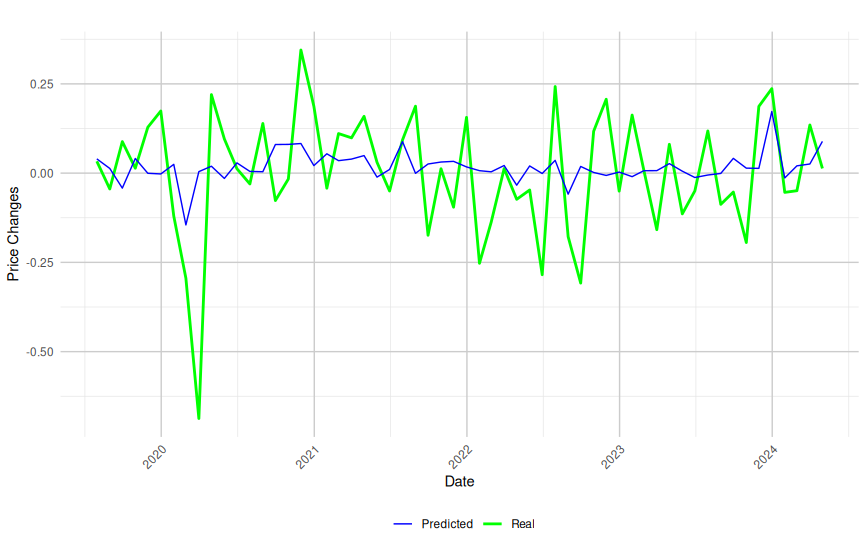
\includegraphics[width=0.8\textwidth]{long-term-monthly.png}
    \caption{Long-term predicted vs monthly real FTSE250 price changes}
    \label{fig:lmonthly}
\end{figure}

The interpretation of this is that, over the long-run (4-5 years), the variations in the 
Consumer Price Index, interest rate, USD/GBP exchange rate, and M3 money 
supply explain or account for $9\%$ of the fluctuations of the
monthly FTSE250 value. This relates closely to the findings of \citeboth{conover1999}, 
who used an econometric model to establish that $4\%$ of the variation in monthly UK stock returns can be 
explained by variations in the money supply. It also suggests a higher level of influence 
than the ARDL-ECM model provided, that only $R^2=3.4\%$ of the monthly FTSE250 variations 
are affected by the selected macroeconomic variables, demonstrating the ability of machine learning
methods to capture subtle patterns in the data unavailable to econometric models. 

\begin{figure}[h]
    \centering
    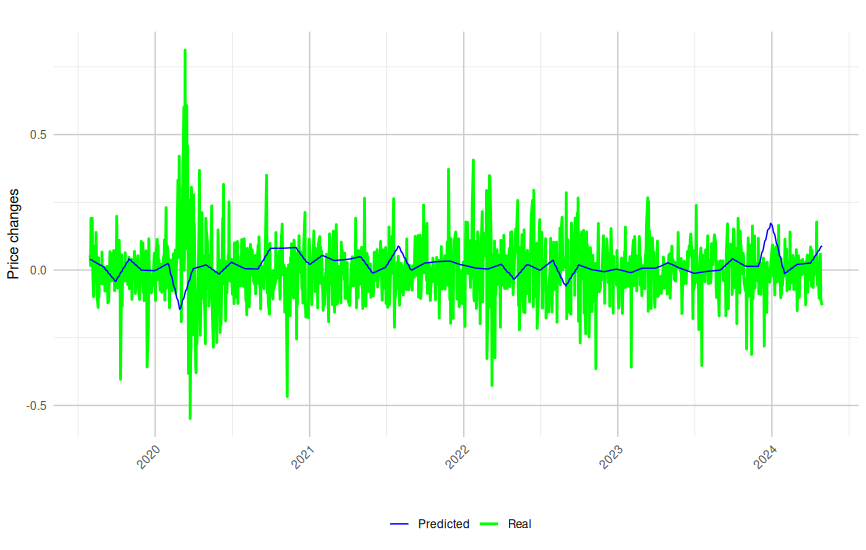
\includegraphics[width=0.8\textwidth]{long-term-daily.png}
    \caption{Long-term predicted vs daily real FTSE250 price changes}
    \label{fig:ldaily}
\end{figure}

In the context of a phenomenon as complex as the stock market,
which is influenced by an inumerable quantity of factors such as investor sentiment
- inherently irrational, 
political instability, geopolitical shocks, corporate governance, and financial regulation, this result 
unsurprising. Furthermore, the selection of economic variables in this study
is by no means exhaustive; commodity prices, international trade dynamics,
economic growth, and many other variables also exert a non-insignificant 
effect on the stock market.

\begin{figure}[h]
    \centering
    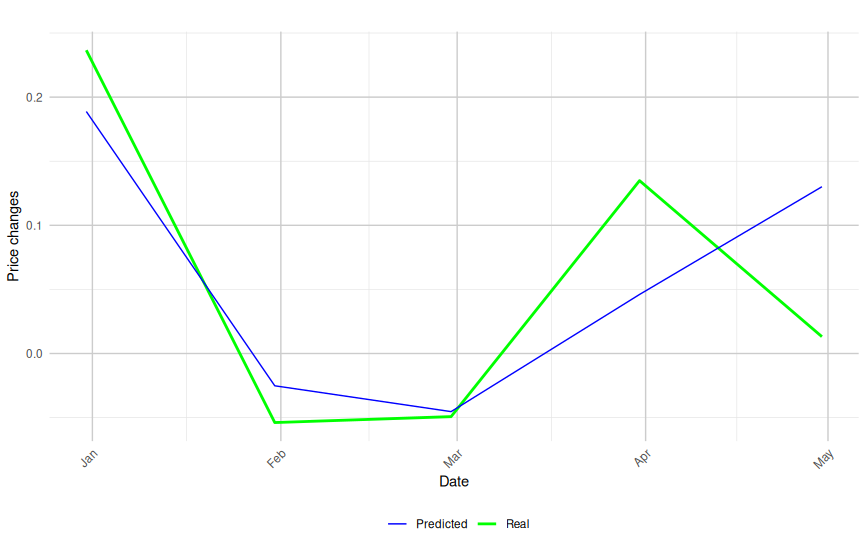
\includegraphics[width=0.8\textwidth]{short-term-monthly.png}
    \caption{Short-term predicted vs monthly real FTSE250 price changes}
    \label{fig:smonthly}
\end{figure}

The short-term prediction yielded MAE = $0.07$ and 
$R^2 = 61\%$, for a 5-month time horizon.
The significantly better performance of the model in the short-run
indicates that the selected macroeconomic variables possesses
a stronger predictive power over shorter periods. This was highlighted 
earlier in the ARDL model, with the interest rate and money supply significantly
impacting the FTSE250 price in the short-run. 

\begin{figure}[h]
    \centering
    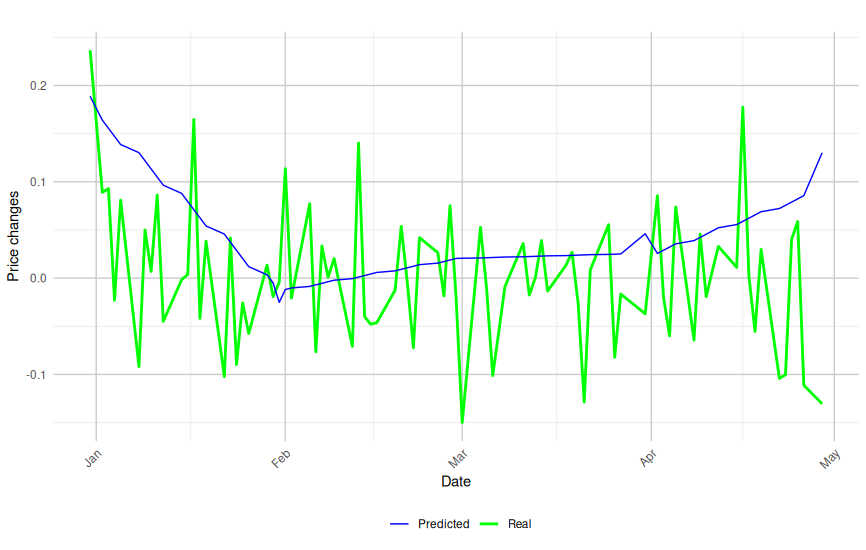
\includegraphics[width=0.8\textwidth]{short-term-daily.png}
    \caption{Short-term predicted vs daily real FTSE250 price changes}
    \label{fig:sdaily}
\end{figure}


In the short-term, which defined as 5 months, 
as per the optimum lag for the FTSE250 in the ARDL model, the market movements
are more closely tied to recent deviations in the economy, because theoretically
the short-run is not exposed to the various unforeseen external shocks and structural changes
that dilute the relationship between these variables and the stock market in the 
long-run. Essentially, as the prediction window expands, 
more uncertainty and unknowns are introduced, which translates into 
lower predictive quality. Furthermore, as the time horizon extends into the long-run, fundamental factors 
begin to matter a lot more. The compound effect of earnings, cash flows and
managerial efficiencies begins to outweigh the 
influence of fluctuating macroeconomic sentiment. Thus, in the short-run 
a different phenomenon is observed.





\section{Conclusion}

Stock markets provide important information on the economy, 
and economic policymakers are vigilant in tracking the fluctuations 
in these markets, and try to forecast the 
forthcoming fluctuations based on policy changes that affect the macroeconomy.
Within this context, the study examined the 
impacts of the interest rate, USD/GBP
exchange rate, the consumer price index, and 
M3 money supply market activity on
the FTSE250 index over the October 1993 – April 2024 period.
The results suggest a cointegrated long-run
relationship between the macroeconomic variables and the stock market index. 
The long-run coefficients imply that
increases in the interest rate and depreciation in the exchange rate
significantly depress the FTSE250 value. 
Policymakers dealing with forecasting the UK stock markets
should consider the factors in the study, and to raise the stock
market's value, a lower interest rate regime should be adopted and 
the Pound should be made more competitive.

The study also investigated the efficacy of machine learning methods in 
the field of stock-econometric forecasting. The RBF-NN performed well in
short-term forecasting of the FTSE250, and offers investors with an accurate forecasting tool, 
to leverage in their trading strategies. The long-term forecast was able to improve on the ARDL-ECM model, and provides 
economists with a tool to compute non-econometric, quantitative measures of the 
long-term influence of macroeconomic variables on the stock market. 

Further research should endeavour to include other macroeconomic variables such as 
foreign direct and portfolio investment, commodity prices and economic growth.
An autoregresive model, falling outside the immediate scope of the current study, could also be tried, including the past values of the 
FTSE250 in the input space to provide a more accurate model. In addition, 
a more granular data set could be utilised by applying a 
Brownian bridge algorithm to generate daily macroeconomic data and 
subsequently testing the RBF-NN against other neural networks 
such as auto-regressive LSTMs, as well as other machine learning methods suited for 
forecasting such as Gradient Boosting Machines and Support Vector Machines. 

\bibliographystyle{plainnat}
\bibliography{paper}

\end{document}
